\documentclass{book}
\usepackage{commeunjeustyle}
\begin{document}
\chapter*{Fonctions de plusieurs variables}
Le cours porte sur les fonctions de plusieurs variables. Prenons un exemple, voici la photographie d'une relief montagneux et sa carte topographique associée :\\
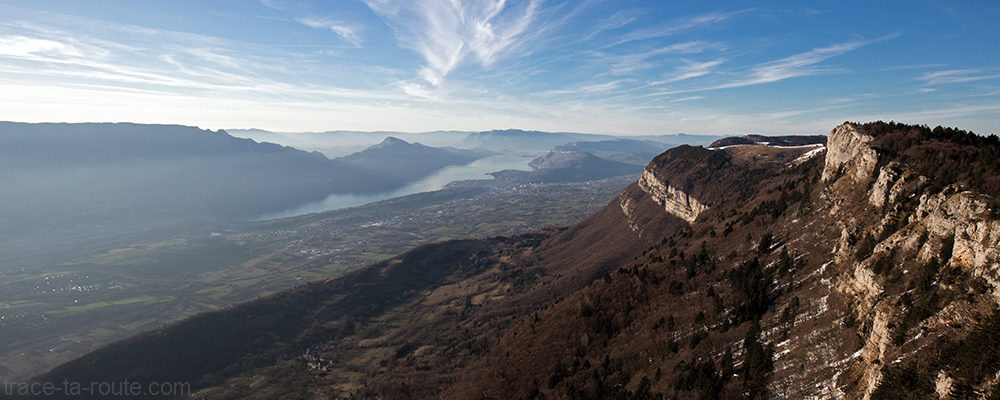
\includegraphics[height=3.5cm]{topography.png}
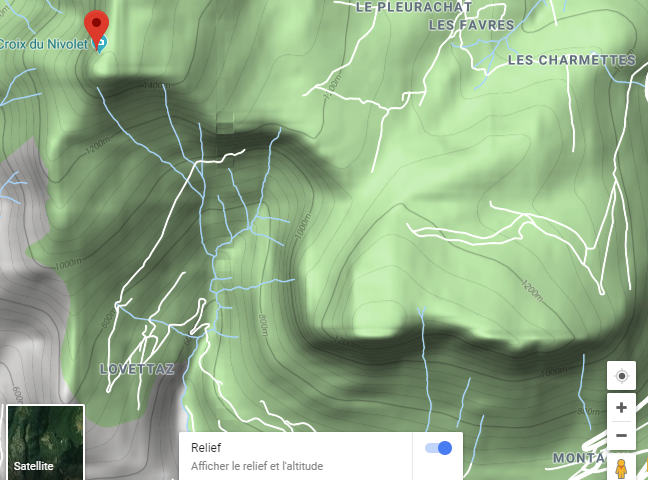
\includegraphics[height=6cm]{topography2.png}.\\
La lecture de la carte de topographique donne l'altitude en fonction de la position définie par la latitude et la longitude, soit une fonction d'un domaine $D$ de $\R^2$ à valeurs dans $\R$.  Par exemple, à l'emplacement de la  Croix de Nivolet (45° 3' 49" nord, 5° 57' 56" soit l'icône de localisation en rouge sur la carte), l'altitude donnée par les courbe de niveaux (points du relief ayant la même altitude) est d'à peu près 1500 mètres. Les falaises représentent des discontinuité de la fonction. Les cols dans la montagne représentent des points critiques qui ne sont pas des extremum car selon une direction, le col apparaît comme un maximum et selon l'orthogonal de cette direction, comme un minimum.     
%\begin{tikzpicture}[scale=0.5]
%    \begin{axis}
%    \addplot3[patch,patch refines=3,
%		shader=faceted interp,
%		patch type=biquadratic] 
%    table[z expr=x^2-y^2]
%    {
%        x  y
%        -2 -2
%        2  -2
%        2  2
%        -2 2
%        0  -2
%        2  0
%        0  2
%        -2 0
%        0  0
%    };
%    \end{axis}
%\end{tikzpicture}\\
L'objet de ce cours est d'étendre l'étude faite sur les fonctions de la variable réel aux fonctions de plusieurs variables.

     
Définitions

Représentation ligne de niveaux graphes voirs cours page 29 http://math.univ-lyon1.fr/~pujo/analyse3.pdf     
     
\end{document}
